\chapter{THE MODEL ATOM FOR ISO-SEQUENCES}
% !TEX root = hazy3.tex

\section{Overview}

\Cloudy\ is designed to model environments that range from the low-density
limit to strict thermodynamic equilibrium.  Eventually all isoelectronic
series will be is treated as a multi-level atom plus continuum.   The
following chapters go over the H-like and He-like sequences.  This chapter
provides an overview.

Following sections are adapted from \citet{Ferland1988}, \citet{Ferland1989}, and \citet{FerlandPeterson1992}.

\section{Departure coefficients}

Departure coefficient is the ratio of the actual population of a state
to its population is thermodynamic equilibrium.  They are useful since they
allow direct comparison of a population to its asymptotic equilibrium limit.

The LTE relative population density for level $n$ is given by
\begin{equation}
\begin{array}{cl}
 {P_n}^*& = \frac{{n_n^*}}{{{n_e}{n_{ion}}}} =
\frac{{{g_n}}}{{{g_e}{g_{ion}}}}{\left(
{\frac{{m_n^*}}{{{m_e}\,{m_{ion}}}}\frac{{{h^2}}}{{2\pi \,kT}}}
\right)^{3/2}}\exp \left( { + {\chi _n}} \right) \\
&  \approx \frac{{{g_n}}}{{{g_e}{g_{ion}}}}{\left( {\frac{{{h^2}}}{{2\pi
\,{m_e}\,kT}}} \right)^{3/2}}\exp \left( { + {\chi _n}} \right) \\
&  = \frac{{{g_n}}}{{{g_e}{g_{ion}}}}4.1412957 \times {10^{ - 16}}{T^{ -
3/2}}\exp \left( { + {\chi _n}} \right) \\
 \end{array}
\mathrm{[cm^3]}
\end{equation}
where the electron statistical weight is $g_e = 2$, the ion statistical weights
are 1 and 2 for H-like and He-like species,
all nuclear statistical weights are ignored,
and $g_n = 2n^2$ is the statistical weight of hydrogenic level $n$.
$n_n*$ is the LTE population of level $n$~[$\pcc$ ],
and the other symbols have their usual meaning.
Here
\begin{equation}
{\chi _n} = \frac{{{I_n}}}{{kT}} = \frac{{15.7807 \times
{{10}^4}{Z^2}}}{{{n^2}T}}
\end{equation}
where $I_n$ is the ionization threshold for level $n$
and Z is the nuclear charge,
the exponent in equation 1 is positive,
and the last term holds for hydrogenic systems.
The dimensionless departure coefficients are related to the LTE
relative population density by
\begin{equation}
b_n = \frac{n_n}{P_n^* n_e n_{ion}}
\end{equation}
where $n_n$ is the actual population of the level.

\section{Pressure lowering of the ionization potential}

Not yet \dots.%[gjf1]

\section{Recombination rates and cooling}

This section is taken from \citet{Ferland1989}.

State-specific rates for radiative recombination and radiative
recombination cooling are needed for the temperature range
\TEMPLIMITLOW$ \le T \le $\TEMPLIMITHIGH.
The methods and assumptions used to derive these for hydrogenic ions
are described here.

\subsection{Formalism}

The Milne relation for the state-specific radiative recombination rate
coefficient (cm$^3$~s$^{-1}$) to a level $n$ can be expressed as
\citep{Brown1970}; \citealp{Gould1978}; \citealp{Mihalas1978});
\begin{equation}
\label{eqn:RecombinCoeffic}
\begin{array}{ccl}
 {\alpha _n}\left( T \right)& =& {\left( {\frac{{2\pi \,{m_e}k}}{{{h^2}}}}
\right)^{ - 3/2}}\frac{{8\pi }}{{{c^2}}}\frac{{{g_n}}}{{{g_e}{g_{ion}}}}{T^{
- 3/2}}\int_{h{\nu _o}}^\infty  {{\nu ^2}{\alpha _\nu }\left( n \right)}
\exp \left( { - h\left( {\nu  - {\nu _o}} \right)/kT} \right)\;d\nu  \\
&  =& 4.12373 \times {10^{11}}\frac{{{g_n}}}{{{g_e}{g_{ion}}}}{T^{ -
3/2}}\int_{h{\nu _o}}^\infty  {{\nu _{Ryd}}^2{\alpha _\nu }\left( n \right)}
\exp \left( { - h\left( {\nu  - {\nu _o}} \right)/kT} \right)\;d{\nu _{Ryd}}
\\
 \end{array}
\end{equation}
where the $g$'s are the statistical weights of the constituents,
$h\nu_{Ryd}$ is the photon energy in Rydbergs,
$h\nu_o \sim z^2/n^2$ is the ionization potential in Rydbergs,
$\alpha_\nu(n)$ is the photoionization cross section,
and the other symbols have their usual meanings.

In implementing this formalism the fact that, for hydrogen itself, the
energy scale is shifted by the ratio of the reduced mass of the nucleus
to an infinite mass was explicitly taken into account.  If the energy of
level $n$ of hydrogen is $n^{-2} R_{\mathrm{H}}$,
then the temperature corresponding to 1 Rydberg,
appearing in the exponential, is 157807~K,
not the commonly quoted 157890~K.
This does affect the results slightly since the energy scale
enters as an exponential in equation~\ref{eqn:RecombinCoeffic}.

Hydrogenic photoionization cross sections are required over a very wide
range of energy since recombination coefficients over a wide range of
temperature are needed.
Cross sections $\alpha_\nu(n)$ were calculated using a program
based on routines developed by \cite{Hummer1988},
\cite{Storey1991}, and Hummer (private communication).
The program generates the cross section values
at arbitrary photon energies for all hydrogenic ($n$,l) states, as well as
for the total $n$, employing analytic expressions and some very accurate
expansions and numerical procedures.  The calculations were carried out
at a number of different mesh sizes to check for convergence.  The results
are typically accurate to better than 0.1 percent.

The recombination cooling rate coefficient (erg cm$^3$~s$^{-3}$)
is given by
\begin{equation}
kT\beta \left( {t,n} \right) = {\left( {\frac{{2\pi {m_e}k}}{{{h^2}}}}
\right)^{ - 3/2}}\frac{{8\pi }}{{{c^2}}}\frac{{{g_n}}}{{{g_e}{g_{ion}}}}{T^{
- 3/2}}\int_{h{\nu _o}}^\infty  {{\nu ^2}\;{\alpha _\nu }\left( n
\right)\;h\left( {\nu  - {\nu _o}} \right)\;\exp \left( { - h\left( {\nu
- {\nu _o}} \right)/kT} \right)\;d\nu }
\end{equation}

\subsection{Results}

%   Table 1
\begin{table}
\label{tab:RecombinCoeffic}
\caption{State Specific and Case B Recombination Coefficients}
\begin{tabular}{llllllll}
\hline
log(T$_e$)& 1&  2&  3&  4&  5&  6&  Case B\\
\hline
0.5& 9.258-12&
5.087-12& 3.512-12& 2.684-12& 2.172-12& 1.825-12& 5.758-11\\
1.0&
5.206-12& 2.860-12& 1.974-12& 1.508-12& 1.220-12& 1.025-12& 2.909-11\\
1.5&  2.927-12& 1.608-12& 1.109-12& 8.465-13& 6.842-13& 5.737-13&
1.440-11\\
2.0& 1.646-12& 9.028-13& 6.216-13& 4.732-13& 3.811-13&
3.183-13& 6.971-12\\
2.5& 9.246-13& 5.055-13& 3.460-13& 2.613-13&
2.084-13& 1.720-13& 3.282-12\\
3.0& 5.184-13& 2.805-13& 1.888-13&
1.395-13& 1.085-13& 8.717-14& 1.489-12\\
3.5& 2.890-13& 1.517-13&
9.779-14& 6.884-14& 5.099-14& 3.912-14& 6.430-13\\
4.0& 1.582-13&
7.699-14& 4.555-14& 2.965-14& 2.053-14& 1.487-14& 2.588-13\\
4.5&
8.255-14& 3.461-14& 1.812-14& 1.076-14& 6.953-15& 4.775-15& 9.456-14\\
5.0& 3.882-14& 1.316-14& 6.059-15& 3.314-15& 2.022-15& 1.331-15&
3.069-14\\
5.5& 1.545-14& 4.196-15& 1.736-15& 8.918-16& 5.219-16&
3.335-16& 8.793-15\\
6.0& 5.058-15& 1.146-15& 4.392-16& 2.160-16&
1.229-16& 7.694-17& 2.245-15\\
6.5& 1.383-15& 2.760-16& 1.005-16&
4.807-17& 2.685-17& 1.660-17& 5.190-16\\
7.0& 3.276-16& 6.031-17&
2.129-17& 1.000-17& 5.523-18& 3.385-18& 1.107-16\\
7.5& 7.006-17&
1.227-17& 4.251-18& 1.976-18& 1.083-18& 6.606-19& 2.221-17\\
8.0&
1.398-17& 2.377-18& 8.139-19& 3.759-19& 2.052-19& 1.248-19& 4.267-18\\
8.5&  2.665-18& 4.455-19& 1.515-19& 6.970-20& 3.796-20& 2.303-20&
7.960-19\\
9.0& 4.940-19& 8.175-20& 2.769-20& 1.271-20& 6.913-21&
4.190-21& 1.457-19\\
9.5& 9.001-20& 1.481-20& 5.005-21& 2.294-21&
1.247-21& 7.552-22& 2.636-20\\
10.0& 1.623-20& 2.662-21& 8.985-22&
4.116-22& 2.235-22& 1.354-22& 4.737-21\\
\hline
\end{tabular}
\end{table}

\begin{table}
\label{tab:RecombinCoolingCoeffic}
\caption{State Specific and Case B Recombination Cooling Coefficients}
\begin{tabular}{llllllll}
\hline
log(T$_e$)& 1&  2&  3&  4&  5&  6&  case B\\
\hline
0.5& 4.025-27&
2.211-27& 1.527-27& 1.167-27& 9.441-28& 7.929-28& 2.295-26\\
1.0&
7.158-27& 3.932-27& 2.713-27& 2.072-27& 1.676-27& 1.406-27& 3.595-26\\
1.5&      1.273-26& 6.985-27& 4.815-27& 3.671-27& 2.962-27& 2.479-27&
5.514-26\\
2.0&      2.262-26& 1.239-26& 8.507-27& 6.451-27& 5.171-27&
4.293-27& 8.236-26\\
2.5 &     4.015-26& 2.184-26& 1.483-26& 1.107-26&
8.708-27& 7.074-27& 1.187-25\\
3.0&      7.099-26& 3.785-26& 2.488-26&
1.784-26& 1.341-26& 1.039-26& 1.629-25\\
3.5&      1.241-25& 6.245-26&
3.796-26& 2.505-26& 1.740-26& 1.255-26& 2.082-25\\
4.0&      2.094-25&
9.195-26& 4.856-26& 2.845-26& 1.795-26& 1.198-26& 2.395-25\\
4.5&
3.234-25& 1.112-25& 4.923-26& 2.557-26& 1.483-26& 9.305-27& 2.376-25\\
5.0&      4.173-25& 1.056-25& 3.990-26& 1.891-26& 1.034-26& 6.240-27&
1.981-25\\
5.5&      4.149-25& 7.981-26& 2.698-26& 1.208-26& 6.389-27&
3.771-27& 1.390-25\\
6.0&      3.121-25& 4.961-26& 1.572-26& 6.827-27&
3.549-27& 2.073-27& 8.316-26\\
6.5&      1.843-25& 2.616-26& 8.015-27&
3.429-27& 1.768-27& 1.028-27& 4.307-26\\
7.0&      9.016-26& 1.204-26&
3.628-27& 1.541-27& 7.917-28& 4.591-28& 1.967-26\\
7.5&      3.847-26&
4.978-27& 1.487-27& 6.296-28& 3.229-28& 1.870-28& 8.109-27\\
8.0&
1.490-26& 1.897-27& 5.644-28& 2.385-28& 1.222-28& 7.077-29& 3.092-27\\
8.5&      5.397-27& 6.811-28& 2.023-28& 8.541-29& 4.375-29& 2.533-29&
1.115-27\\
9.0&      1.867-27& 2.346-28& 6.959-29& 2.937-29& 1.504-29&
8.706-30& 3.872-28\\
9.5&      6.261-28& 7.849-29& 2.327-29& 9.820-30&
5.028-30& 2.910-30& 1.316-28\\
10.0&      2.057-28& 2.575-29& 7.633-30&
3.220-30& 1.649-30& 9.543-31& 4.436-29\\
\hline
\end{tabular}
\end{table}

The numerical results are presented in Tables \ref{tab:RecombinCoeffic}
and \ref{tab:RecombinCoolingCoeffic}.
The first column
of the table gives the log of the temperature.  Columns 2 through 7 give
the total recombination coefficient for $1 \le n \le 6$ summed over $l$ states. The
last column gives the case B sum, $2\le  n\le  1000$.  A very large temperature
range is considered for completeness; actually, at very low temperatures
three-body recombination predominates for most densities
\citep{Bates1962},
while at very high temperatures other processes (i.e., Compton scattering,
collisions) dominate the balance and the neutral fraction is vanishingly
small.

As tests, these predictions of the recombination rate coefficients are
compared with those of \citep{Seaton1959a},
\citep{Ferland1980c}, \citep{Hummer1987}, and \citet{Martin1988}.
Note that the total recombination rate given
by Hummer and Storey is the sum of radiative and net three-body
recombination.  For this comparison their results for a density of
$10^2 \pcc$
were used to minimize the contribution of the second process.  The agreement
with all of these results is good, usually much better than 1 percent.
\citep{Seaton1959a} calculates the recombination cooling coefficients.
The present
results agree with his to better than 5 percent.
Figure \ref{fig:HRecomCooling} shows the recombination-cooling coefficient for several states.

\begin{figure}
\label{fig:HRecomCooling}
\centering
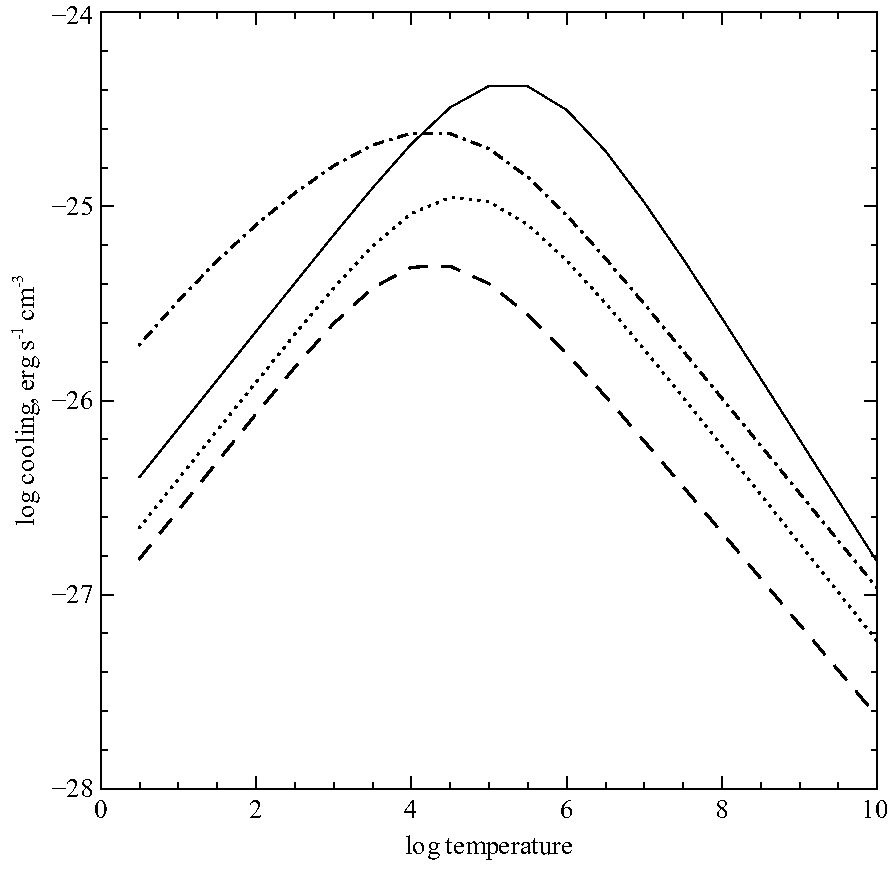
\includegraphics[scale=0.8]{HRecomCooling}
\caption[H recombination cooling]{The recombination cooling for several states is shown as a function
of temperature.}
\end{figure}

\section{The collisional rate equations}

The collision rates between two terms in strict
thermodynamic equilibrium (STE) are related by detailed
balance.  Then
\begin{equation}
n_l^*{C_{l,u}} = n_u^*{C_{u,l}}
\end{equation}
and we get the usual relation between collisional excitation and
de-excitation rates,
\begin{equation}
{C_{l,u}} = \left( {n_u^*/n_l^*} \right){C_{u,l}} = \left( {{g_u}/{g_l}}
\right)\exp \left( { - \chi /kT} \right){C_{u,l}}.
\end{equation}

Considering only collisional terms, the departure coefficient for level
$n$ is given by
\begin{equation}
\frac{{d{b_n}}}{{dt}} = \sum\limits_l {{b_l}{C_{n,l}} + \sum\limits_u
{\frac{{P_u^*}}{{P_n^*}}{b_u}{C_{u,n}} - {b_n}\left\{ {\sum\limits_l
{{C_{n,l}}}  + \sum\limits_u {\frac{{P_u^*}}{{P_n^*}}{C_{u,n}} +
{C_{n,k}}\left( {1 - b_n^{ - 1}} \right)} } \right\}} }
\end{equation}
where the sums are over upper and lower levels.
The collision rates
($\ps$)
from level $i$ to level $j$ are denoted by $C_{ij}$.
The first term on the RHS
represents collisional excitation to $n$ from lower levels, the second is
collisional deexcitation to $n$ from higher levels,
and the last term accounts
for destruction processes.
These include collisions to lower levels, upper
levels, and the continuum.
The factor multiplying the collisional ionization
rate $C_{n\kappa}$ accounts for collisional ionization less three-body recombination.
Note that this is often a net recombination process for the atom since,
under many circumstances, $b_n < 1$.

Figure \ref{fig:HDepartCoefVsDensity} shows a test case where collisional processes are dominant.
All of the radiative processes discussed below are actually included, but
the intensity of the external continuum is set to a very low (and hence
negligible) value.  As a result collisional and spontaneous radiative
processes are dominant.  The electrons are given a temperature of 50000
K, and the level populations and ionization of the gas are determined by
solving the full set of equations of statistical equilibrium.  The model
is of a very thin cell of gas that is optically thin in the lines and
continuum.  Departure coefficients for the ground state, 2s, 2p, and 4 are
shown.

\begin{figure}
\label{fig:HDepartCoefVsDensity}
\centering
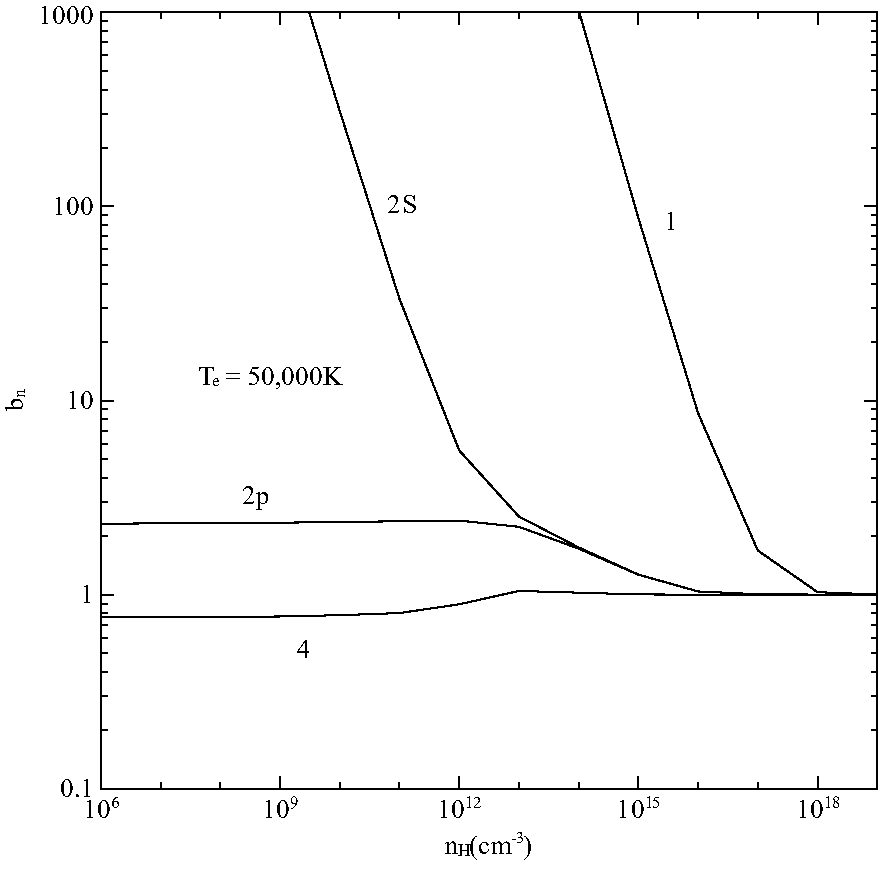
\includegraphics[scale=0.8]{HDepartCoefVsDensity}
\caption[H populations vs density]{The equilibrium populations of the ground state and levels  $2s$,
$2p$, and 4 of the model hydrogen atom
are shown as a function of the total
hydrogen density n$_{\mathrm{H}}$.}%
\end{figure}

The radiation field is set to a very low intensity, and the column density
is kept small enough for optical depth effects to be negligible.  A constant
electron temperature of $5\times  10^4 \K$ is assumed, so the gas is primarily
collisionally ionized and excited.
Levels $2s$ and $2p$ do not mix until a
density of nearly $10^{14} \pcc$ is reached,
and do not come into LTE until the
density is nearly 100 times higher.
The entire atom is nearly in LTE at
densities greater than $10^{18} \pcc$

The ground state is overpopulated relative to its LTE value when upward
collisional processes are much slower than downward radiative processes.
It is only when the collisional rates approach the radiative rates that
$b_1$ approaches unity.
The $2s$ level also has a large overpopulation for much
the same reason.  It is highly metastable and accumulates a large
overpopulation until $2s -- 2p$ collisions become fast enough
to mix the two $l$ levels.
The more highly excited levels ($n\ge  3$) have a behavior very similar
to that of $n=4$, which is shown in the figure.  They are under populated
relative to their LTE value when radiative decays to lower levels are
competitive with collisional processes.
It is only at a density of $n_H > 10^{18} \pcc$ that collisional processes completely dominate the rate equations
and the atom reaches LTE.
The mean departure coefficient at a density of
$10^{19} \pcc$ is ${\bar b_i} = 1.0007 \pm 0.0022$
for the entire atom, and the largest single deviation from unity is
0.7\% (for the ground level).

\section{The radiative rate equations}

\subsection{Photoionization---recombination}

The photoionization rate ($\ps$) is given by
\begin{equation}
{\Gamma _n} = 4\pi \,\int_{{\nu _o}}^\infty  {\frac{{{J_\nu }}}{{h\nu
}}\;{\alpha _\nu }\;d\nu }\quad [\mathrm{s}^{-1}]
\end{equation}
and the induced recombination rate coefficient by
\begin{equation}
\label{eqn:InducedRecombinationRateCoefficient}
\alpha \left( {ind} \right) = P_n^*4\pi \int_{{\nu _o}}^\infty
{\frac{{{J_\nu }}}{{h\nu }}\;{\alpha _\nu }\exp \left( { - h\nu /kT}
\right)\;d\nu }\quad  [\mathrm{cm}^3 \mathrm{s}^{-1}].
\end{equation}
This is evaluated at each zone by direct integration.

The ground level also includes destruction due to bound Compton scattering.

\subsection{Derivation of radiative balance equations}

Consider the balance for a level $n$ of a three level system, with upper
and lower levels $u$ and~$l$.
\begin{equation}
{n_n}\left( {{B_{n,u}}\bar J + {B_{n,l}}\bar J + {A_{n,l}}} \right) =
{n_u}\left( {{B_{u,n}}\bar J + {A_{u,n}}} \right) + {n_l}{B_{l,n}}\bar J.
\end{equation}
Converting densities ni into departure coefficients, ${n_i} = {b_i}P_i^*$, we obtain
\begin{equation}
P_n^*{b_n}\left( {{B_{n,u}}\bar J + {B_{n,l}}\bar J + {A_{n,l}}} \right)
= P_u^*{b_u}\left( {{B_{u,n}}\bar J + {A_{u,n}}} \right) +
P_l^*{b_l}{B_{l,n}}\bar J.
\end{equation}
Gathering LTE densities we find
\begin{equation}
{b_n}\left( {{B_{n,u}}\bar J + {B_{n,l}}\bar J + {A_{n,l}}} \right) =
\frac{{P_u^*}}{{P_n^*}}{b_u}\left( {{B_{u,n}}\bar J + {A_{u,n}}} \right)
+ \frac{{P_l^*}}{{P_n^*}}{b_l}{B_{l,n}}\bar J.
\end{equation}
Writing $B_{ln} = B_{nl} g_n/g_l$, we obtain the final form
\begin{equation}
{b_n}\left( {\frac{{{g_u}}}{{{g_n}}}{B_{u,n}}\bar J + {B_{n,l}}\bar J
+ {A_{n,l}}} \right) = \frac{{P_u^*}}{{P_n^*}}{b_u}\left( {{B_{u,n}}\bar
J + {A_{u,n}}} \right) +
\frac{{P_l^*}}{{P_n^*}}{b_l}\frac{{{g_n}}}{{{g_l}}}{B_{n,l}}\bar J.
\end{equation}

\subsection{Final radiative equations}

The full set of radiative balance equations can be written as
\begin{equation}
\begin{array}{ccc}
 \frac{{d{b_n}}}{{dt}}& = & \sum\limits_l
{\frac{{P_l^*}}{{P_n^*}}{b_l}{A_{n,l}}\frac{{{g_n}}}{{{g_l}}}\,{\eta
_{n,l}}{\gamma _{n,l}} + \sum\limits_u {\frac{{P_u^*}}{{P_n^*}}{b_u}\left(
{{A_{u,n}}{P_{u,n}} + {A_{u,n}}{\eta _{u,n}}{\gamma _{u,n}}} \right)} }
+  \\
&&
 \left[ {\alpha \left( {rad} \right) + \alpha \left( {ind} \right)}
\right]/P_n^* -  \\
&&
 {b_n}\left( {\sum\limits_l {\left( {{A_{n,l}}{P_{n,l}} + {A_{n,l}}{\eta
_{n,l}}{\gamma _{n,l}}} \right) + \sum\limits_u
{{A_{u,n}}\frac{{{g_u}}}{{{g_n}}}{\eta _{u,n}}{\gamma _{u,n}} + {\Gamma
_n}} } } \right) \\
 \end{array}
\end{equation}
where the $\eta$ is the continuum occupation number in the transition $ij$.

Figure \ref{fig:HDepartCoefVsRadiationField} shows a test case that,
in contrast to that shown in Figure
\ref{fig:HDepartCoefVsDensity},
is dominated by radiative transitions.

\begin{figure}
\label{fig:HDepartCoefVsRadiationField}
\centering
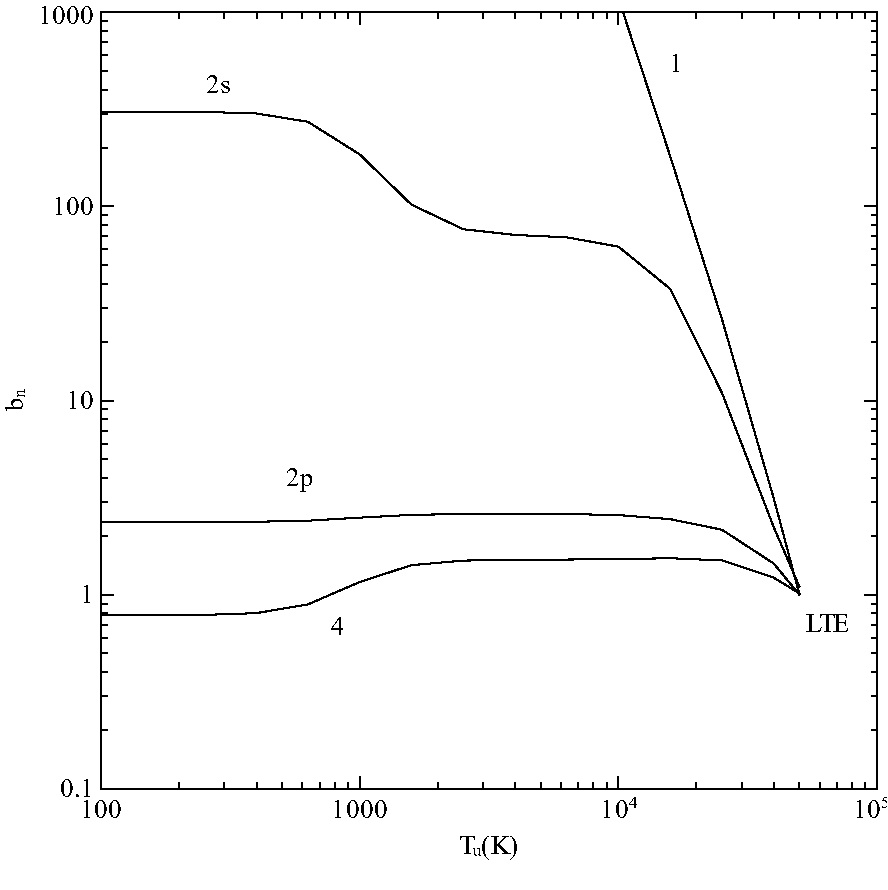
\includegraphics[scale=0.8]{HDepartCoefVsRadiationField}
\caption[H populations vs radiation field]{The calculations are for a constant temperature $(T = 5 \times
10^4 K)$
optically thin gas exposed to black body radiation with a color temperature
of $T_{color} = 5 \times 10^4 K$, but with various values of the energy density,
parameterized as $T_u = (u/a)^{1/4}$, where u is the actual radiation
density.}
\end{figure}

Again, the full set of equations coupling the levels are solved, but
spontaneous and induced processes are more important than collisions for
many values of the radiation density.  The model is of a very thin cell
of gas, so that all lines and continua are optically thin, has a density
of $n(H) = 10^{10}$~cm$^{-3}$, and an electron temperature of $5 \times
10^4$~K.
The gas is
exposed to a black body continuum with a color temperature of
$T_{color} = 5
\times 10^4$~K, but the intensity of this continuum is varied.  This intensity is
parameterized by an energy density temperature defined by $T_u \equiv
(u/a)^{1/4}$ where
$u$ and $a$ are, respectively, the actual radiation energy density and Stefan's
radiation density constant.

A radiation field given by Planck's law (i.e., $T_u\equiv  T_{color}$) forces the
ionization and level population of an atom or ion to LTE in much the same
way that high electron densities do.
As Figure \ref{fig:HDepartCoefVsRadiationField} shows, at very low values
of $T_u$ (low photon densities) the ground and $n = 2$ states are overpopulated
for much the same reason that this occurs at low electron densities; the
downward spontaneous radiative rates are fast relative to the induced (upward
and downward) rates.  At very low $T_u (< 500 \K), n \ge 3$ levels are under
populated since they decay at a rate much faster than the induced rates
(for $T = 5 \times 10^4$~K these levels have $h\nu? kT$, so induced processes will be
fast relative to spontaneous rates when $T_u = T_{color}$ and the atom is in LTE).
As $T_u$ increases, fluorescence from the ground state over-populates excited
states (because the ground state is itself overpopulated) and $b_4$ exceeds
unity.  Finally, in the limit where $T_u = T_{color}$, the departure coefficients
reach unity and the atom goes to LTE.  (The actual mean departure coefficient
for the entire atom is ${\bar b_i} = 1.013 \pm 0.029$).  Note that the vast majority of the neutral hydrogen population is
in excited states when the atom approaches LTE at these temperatures.

The hydrogen density $(n(H) = 10^{10}$~cm$^{-3}$) is low enough for radiation to
be the main agent affecting level populations for most values of $T_u$.
Fluorescence from the ground state drives the population of $n=4$ above its
LTE value for many radiation densities.  Induced processes, mainly
transitions between adjacent levels, drive the atom to LTE when $T_u$ reaches
$5 \times 10^4$~K.


